\documentclass{article}

\usepackage{graphicx}
\usepackage{amsmath}
\usepackage{float}
\usepackage{amsfonts}
\usepackage{listings}
\usepackage{xcolor}
\usepackage[utf8]{inputenc}
\usepackage{hyperref}
\usepackage{verbatim}
\usepackage{fancyhdr}

\usepackage[a4paper, margin=1in]{geometry}

\pagestyle{fancy} % Utilise le style fancy
\fancyhf{} % Efface les en-têtes et pieds de page par défaut
\fancyhead[L]{MARIAC Damien, SCAIA Mattéo} % Gauche
\fancyhead[R]{HAX711X} % Droite
\fancyfoot[C]{\thepage} % Numérotation centrée dans le pied de page

\lstset{
  language=R,
  basicstyle=\ttfamily\small,
  numbers=left,               % Numérotation des lignes
  numberstyle=\tiny\color{gray}, % Style de la numérotation
  keywordstyle=\color{blue},  % Couleur des mots-clés
  commentstyle=\color{green}, % Couleur des commentaires
  stringstyle=\color{red},    % Couleur des chaînes de caractères
  breaklines=true,            % Coupe les lignes trop longues
  frame=single,               % Encadre le code
}


\title{TP1 ADM}
\author{MARIAC Damien, SCAIA Matteo}
\date{\today} 

\begin{document}

\maketitle

\begin{figure}[h] 
    \centering
    
\includegraphics[width=0.5\textwidth]{ssd_logo.png} 
\end{figure}

\begin{figure}[h] 
    \centering
    
\includegraphics[width=0.5\textwidth]{logo_um_2022_rouge_RVB.png} 
\end{figure}

\newpage

\tableofcontents

\newpage

\section{Introduction}
Nous disposons d'une base de données comprenant l'analyse de 27 espèces d'arbres réparties dans 1000 parcelles forestières situées dans la forêt du Congo.
Il s'agit d'étudier la variabilité des densités de peuplement d'espèces arborées dans différentes parcelles de la forêt.  Nous avons enlevé une ligne problématique dans notre jeu de données (ligne 1000 code TGC).
Nous disposons dans notre jeu de données de 28 variables quantitatives dont : 27 variables de comptage sur les espèces d'arbres et une sur la surface de la parcelle. De plus, notre base de données intègre deux variables qualitatives : l'une décrivant le type forestier et l'autre le type géologique.
\\
On arrondira nos calculs à $10^{-3}$.


\begin{table}[H]
    \caption{Extrait du jeu de données Datagenus}
    \centering
    \begin{tabular}{|l|l|l|l|l|l|l|}
    \hline
    code & gen1 & gen2 & gen3 & forest & geology & surface \\ \hline
    1299 & 0    & 0    & 0    & 2      & 3       & 5       \\ \hline
    2644 & 9    & 0    & 3    & 7      & 6       & 15      \\ \hline
    1838 & 9    & 0    & 0    & 5      & 6       & 17.5    \\ \hline
    534  & 0    & 4    & 0    & 1      & 5       & 20.5    \\ \hline
    3213 & 1    & 1    & 0    & 1      & 6       & 10.5    \\ \hline
    1861 & 19   & 3    & 1    & 7      & 3       & 20      \\ \hline
    \end{tabular}
\end{table}



\section{Partie 1}
\subsection{Inertie et barycentre}

Afin d'avoir une comparaison plus juste entre chaque parcelle, nous utilisons la densité de peuplement de ces dernières. C'est-à-dire que la densité de peuplement de chaque espèce d'arbre par unité de surface est donnée par :
\[
d^j_i = \frac{n^j_i}{S_i}
\]
où $n^j_i$ est le nombre d'arbres de l'espèce $j$ présents sur la parcelle $i$, et $S_i$ représente la surface de la parcelle $i$.

Nous devons de plus centrer et réduire les variables quantitatives dans le but de mieux comparer celles qui décrivent les différentes densités. Nous allons alors utiliser :
\[
(x^j_i)_{1 \leq j \leq 27} = \frac{x^j_i - \bar{x}_j}{\sigma_j}
\]
avec $\bar{x}_j$ la moyenne pour la $j$-ème variable et $\sigma_j$ l'écart-type de la $j$-ème variable.

Dans la suite, nous ne considérerons plus que les variables centrées-réduites.

De plus, on supposera que le poids de nos parcelles est équipondéré.
\vspace{2\baselineskip}
\\
\textbf{Par conséquent, on a :}
\\
\\
\indent\underline{Barycentre à l'origine :} (preuve théorique)
\\
\\
Supposons que nous avons un ensemble de données \(X\) composé de \(n\) observations et \(p\) variables (dans notre cas 1000 et 27). Après le centrage et la réduction, les coefficients de notre matrice transformée \(X'\) sont définis par :
\[
x'_{ij} = \frac{x_{ij} - \bar{x}_j}{s_j}
\]
Le barycentre de \(X\) est donné par la moyenne de chaque colonne de \(X\). Calculons cette moyenne pour n'importe quelle \(j\) :
\[
\bar{x}_j = \frac{1}{n} \sum_{i=1}^n \left( \frac{x_{ij} - \bar{x}_j}{s_j} \right) = \frac{1}{s_j} \left( \frac{1}{n} \sum_{i=1}^n x_{ij} - \bar{x}_j \right) = 0
\]
Ainsi, le barycentre de chaque variable dans \(X'\) est zéro.
\\


\underline{Inertie totale égale à 27 : } (preuve théorique)
\\
\\
Considérons la même matrice de données \(X'\). L'inertie de l'ensemble des points \(X\) par rapport à leur barycentre \(y\) est définie par :
\[
I_{y,w} = \sum_{i=1}^n w_i \|x_i - y\|^2
\]
Dans notre cas, le barycentre est nul. De plus, tous les poids \(w_i\) sont égaux (par exemple, \(w_i = \frac{1}{n}\) ce qui est notre cas), alors l'inertie devient :
\[
I_{y,w} = \sum_{i=1}^n w_i \|x_i\|^2 = \frac{1}{n} \sum_{i=1}^n \|x_i\|^2
\]
Comme chaque \(x_i\) est une observation centrée-réduite et la variance de chaque variable est 1, nous avons (pour \(i\) fixé) :
\[
\|x_i\|^2 = \sum_{j=1}^p (x'_{ij})^2 = p
\]
Ainsi, l'inertie totale est :
\[
I_{y,w} = \frac{1}{n} \sum_{i=1}^n p = p
\]
Dans notre cas vaut 27.

\subsection{Autour des types forestiers}

Dans cette section, nous calculons les barycentres des sept types forestiers présents dans les données, ainsi que l'inertie inter-types et le coefficient $R^2$
 associé à la partition des parcelles selon ces types. Ce calcul nous permet d'évaluer la proportion de la variabilité totale des densités de peuplement.


\subsubsection{Calcul des poids des types forestiers}
Le poids de chaque type forestier est calculé comme la proportion de parcelles appartenant à ce type par rapport à l'ensemble des 1000 parcelles. C'est à dire, le poids est donné par :

\[
p_i = \frac{\text{Nombre de parcelles du type } i}{1000}
\]

\begin{table}[H]
    \center
    \caption{Tableau des poids forestiers}
    \begin{tabular}{|l|l|l|l|l|l|l|}
    \hline
    1     & 2     & 3     & 4     & 5     & 6     & 7     \\ \hline
    0.278 & 0.105 & 0.022 & 0.018 & 0.169 & 0.095 & 0.313 \\ \hline
    \end{tabular}
    \end{table}


\subsubsection{Calcul des barycentres des types forestiers}
Pour chaque type forestier $i$,  (avec $X$ la matrice des densités centrées réduites), le barycentre vaut :

\[
\bar{X}_i = \frac{1}{n_i} \sum_{j \in \text{Type } i} X^j
\]

Avec $n_i$ le nombre de parcelles dans le type forestier i.
\\
Nous obtenons alors une matrice $B \in \mathcal{M}_{7,27}(\mathbb{R})$


\subsubsection{Calcul des normes euclidiennes carrées}
Une fois les barycentres calculés, nous évaluons la distance de chaque barycentre à l'origine:

\begin{table}[H]
    \centering
    \caption{normes carrées}
    \begin{tabular}{|l|l|l|l|l|l|l|l|}
    \hline
    type forestier       & 1         & 2         & 3         & 4      & 5     & 6     & 7     \\ \hline
    distance (en norme 2) & 0.772 & 3.228 & 4.279 & 21.210 & 1.092 & 1.443 & 1.628 \\ \hline
    \end{tabular}
    \end{table}

\subsubsection{Inertie inter-types et coefficient $R^2$}
\label{subsec : Inertie inter-types et coefficient}


L'inertie inter-types forestiers est calculée en pondérant les normes euclidiennes carrées par les poids des types forestiers. Elle mesure la variabilité des densités de peuplement expliquée par la partition en types forestiers et elle est définie par :

\[
\text{Inertie inter-types} = \sum_{i=1}^{7} p_i \|\bar{X}_i\|^2 = 1.860
\]

Le coefficient $R^2$ nous permet d'évaluer dans quelle mesure les types forestiers expliquent la variabilité des densités de peuplement dans les parcelles observées.
\[
R^2 = \frac{\text{Inertie inter-types}}{\text{Inertie totale}}=0.069
\]

Cela correspond à une disparité d'environ 7\%

\subsection{Liaisons}

On s'intéresse maintenant à l'interprétation des résultats trouvés. Nous calculons alors le \( R^2 \) de chaque variable densité avec $R^2 = \frac{variance_{inter -typesforestiers}}{variance totale}$.
(C'est à dire : \( R^2 = \frac{\text{Inertie externe}}{\text{Inertie totale}} \).)

\begin{table}[H]
    \centering
    \caption{Extrait du R² des variables}
    \label{tab:statistiques Partie1 a rap avec II.1.b}
    \begin{tabular}{|l|l|l|l|l|}
    \hline
    Especes & gen1  & gen6  & gen17 & gen25 \\ \hline
    R²      & 0.072 & 0.008 & 0.096 & 0.184 \\ \hline
    \end{tabular}
    \centering
\end{table}


    Nous remarquons numériquement que la variable la plus liée au type est gen25, tandis que la moins liée est gen6. 
    \\
    Montrons que le \( R^2 \) de la partition est la moyenne (arithmétique) des \( R^2 \) des densités:

\[
R^2 = \frac{\text{Inertie externe}}{\text{Inertie totale}}
= \frac{1}{27} \sum_{k=1}^{7} \lVert x_k^j \rVert^2
= \frac{1}{27} \sum_{k=1}^{7} \sum_{j=1}^{27} (x_k^j)^2
= \frac{1}{27} \sum_{j=1}^{27} \sum_{k=1}^{7} (x_k^j)^2
= \frac{1}{27} \sum_{j=1}^{27} R_j^2
\]

On retrouve bien numériquement la même valeur :
\\
\begin{lstlisting}[caption=Extrait du code R, label= Question 1b]
    R2_global <- sum(R2_variables) / length(R2_variables)
    print(R2_global)
    
    R2_partition <- sum(poids * rowSums(barycentres_types^2)) / 27
    print(R2_partition)
\end{lstlisting}

\begin{figure}[H]
    \centering
    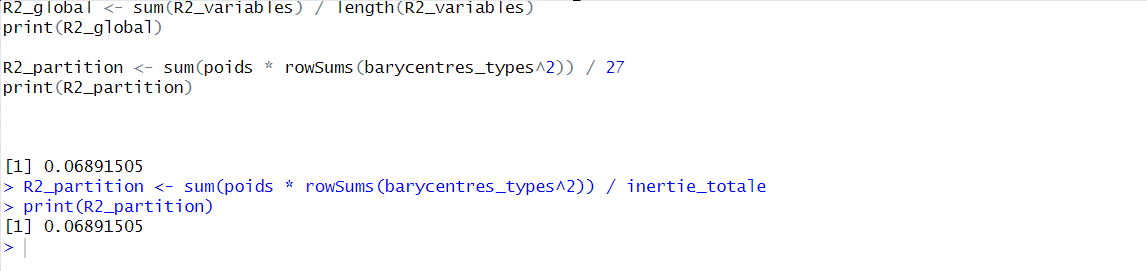
\includegraphics[width=1.5\textwidth]{preuve_info_p1.png}
\end{figure}


\newpage
\section{Partie 2}
\subsection{Enoncer}
On notera $X$ la matrice dont les colonnes sont les 27 densités centrées-réduites, $Y$ la
matrice dont les colonnes sont les indicatrices de types forestiers, et $Z$ celle dont les
colonnes sont les indicatrices de sols (geology). \\
On notera $W=\frac{1}{n}I_n$ la matrice des poids des individus et $M=\frac{1}{p}I_p$
celle des poids des variables.
\subsection{Rappel et calcul de projecteur}
\subsubsection{Rappel}
Montrons l'égalité suivante. \\
\[
\forall j \hspace{0.5cm} \Pi_Y x^j = \Pi_{Y^c} x^j
\]
Nous rappelons que 
\[
Y^c = \Pi_{1^\perp} Y 
\]
\[
\Pi_Y = \Pi_{Y^c} + \Pi_1
\]
A partir de ces deux résultats, nous avons : \\
\begin{align*}
    \Pi_Y x^j & = \Pi_{Y^c} x^j + \Pi_1 x^j \\
    &= \Pi_{Y^c} x^j
\end{align*}
C'est à dire, pour tout $j$ : 
\[
\Pi_Y x^j = \Pi_{Y^c} x^j
\]
De plus, nous avons l'expression suivante.
\[
\left\lVert \Pi_Y x^j \right\rVert^2 _W = \left\langle \Pi_Y x^j,\Pi_Y x^j\right\rangle_W
\]
Or,
\[
\Pi_Y x^j=\sum_{q = 1}^{p}\Pi_{y^q} x^j=\sum_{q = 1}^{p}y^q( \overline{x^j}^q - {\overline{x^j}} )  
\]
Avec, $\overline{x^j}$ représentant la moyenne globale des $x^j$, $\overline{x^j}^q$ représentant la moyenne pondérée des $x^j$ pour le type forestier $q$.\\
A partir de ces notations, nous avons l'expression suivante.
\begin{align*}
    \left\lVert \Pi_Y x^j \right\rVert^2 _W &= \left\langle \Pi_Y x^j,\Pi_Y x^j\right\rangle_W \\
     &=  \sum_{q = 1}^{p}( \overline{x^j}^q - {\overline{x^j}} ) \sum_{ i= 1}^{p}( \overline{x^j}^i - {\overline{x^j}} )\left\langle y^q,y^i\right\rangle_W \\
     &= \sum_{q = 1}^{p}w^q( \overline{x^j}^q - {\overline{x^j}} )^2
\end{align*}
Ici, $\left\lVert \Pi_Y x^j \right\rVert^2 _W$ s'interprète statistiquement comme
étant une mesure pondérée de la variation des $x^j$ dans un certain type forestier.
\\
\\
\subsubsection{Calcul de projecteur}
Le but de cette question est de trouver l'expression
de $\Pi_Y$ et de calculer pour tout $j \in [1,27]$, $\Pi_{x^{j}}$ et $tr(\Pi_{x^{j}}\Pi_Y)$. Nous ferons la démonstration
puis nous programmerons le résultat. \\
Tout d'abord, on rappelle que :
\[
\Pi_Y = Y(Y'WY)^{-1}Y'W
\]
Soit $j \in [1,27]$. Calculons les deux expressions données précédemment.
\[
\Pi_{x^j}= x^{j}(x^{j\prime}Wx^{j})^{-1}x^{j\prime}W
\]
En utilisant les propriétés de la trace et l'expression de $\Pi_{x^j}$, il en suit 
\begin{align*}
    tr(\Pi_{x^{j}}\Pi_Y) &= tr(x^{j}(x^{j\prime}Wx^{j})^{-1}x^{j\prime}W\Pi_Y) \\
    &=tr((x^{j\prime}Wx^{j})^{-1}x^{j\prime}W\Pi_Yx^{j})\\
    &=(x^{j\prime}Wx^{j})^{-1}x^{j\prime}W\Pi_Yx^{j}\\
    &= \frac{\left\langle x^{j\prime},\Pi_Yx^{j}\right\rangle_W }{\left\lVert x^j\right\rVert^2_W }\\
    &= R^2(x^j\mid Y )
\end{align*}
Donc $tr(\Pi_{x^{j}}\Pi_Y)$ représente le $R^2$ d'une densité de population sachant son type forestier. C'est-à-dire que nous 
mesurons la variabilité d'une espèce liée à un type forestier. \\
Nous pouvons programmer les deux expressions ci dessus. \\
\begin{lstlisting}[caption=Extrait du code R, label= Question 1b]
P_Y <- Y %*% solve(t(Y)%*% W %*% Y) %*% t(Y) %*% W
P_X <- function(j){
    # Calculer la projection de la colonne j de X
    x_j <- X[, j, drop = FALSE]  # Pour que x_j reste une matrice
    return(x_j %*% solve(t(x_j) %*% W %*% x_j) %*% t(x_j) %*% W)
}
#On calcule la trace du produit matriciel
Tr_1 <- sum(diag(P_X(3) %*% P_Y))
\end{lstlisting}
Nous effectuons le calcul de la trace pour tout $j \in [1,27]$. Nous obtenons le tableau suivant. 
\begin{table}[H]
    \centering
    \caption{Extrait du $R^2$ des variables via le calcul de la trace}
    \label{tab:statistiques 1.b}
    \begin{tabular}{|l|l|l|l|l|}
    \hline
    Especes & gen1  & gen6  & gen17 & gen25 \\ \hline
    R²      & 0.072 & 0.008 & 0.096 & 0.184 \\ \hline
    \end{tabular}
    \centering
\end{table}

\subsubsection{Calcul de $R$ et de $tr(R\Pi_Y)$ }
\label{subsec:Question 1.c}
De la même manière, nous programmons la matrice $R=XMX'W$, ainsi que $tr(R\Pi_Y)$.
\begin{lstlisting}[caption=Extrait du code R, label= Question 1c]
    R <- X %*% M %*% t(X) %*% W
    Tr_2 <- sum(diag(R %*% P_Y))
\end{lstlisting}
Nous pouvons alors calculer la trace de la matrice demandée et nous obtenons.
\begin{center}
    $tr(R\Pi_Y)=0,069$
\end{center}
Nous pouvons interpréter $tr(R\Pi_Y)$ comme étant le coefficient $R^2$ suivant.
\begin{center}
    $R^2 = \frac{\text{Inertie inter-types}}{\text{Inertie totale}}$
\end{center}
\subsubsection{Interprétation des résultats }
Nous avons trouvé les mêmes résultats que dans la partie 1 du TP. Cependant, dans cette partie, nous avons utilisé des calculs différents.\\
Nous pouvons rapprocher les résultats obtenus dans \autoref{tab:statistiques Partie1 a rap avec II.1.b} et dans \autoref{tab:statistiques 1.b}. En effet, nous avons bien
les mêmes valeurs. De plus, les résultats du coefficient $R^2$ obtenu dans la partie \ref{subsec:Question 1.c} et celui obtenu dans la partie \ref{subsec : Inertie inter-types et coefficient} sont bien identiques.
\\En conclusion, avec deux méthodes de calcul différents, nous retrouvons bien les mêmes résultats.
\subsection{Rapprochement avec la variable "geology"}
Dans cette question, nous allons nous intéresser a la variable $Z$ "geology". Programmons de la même manière, les matrices demandées.
\begin{lstlisting}[caption=Extrait du code R, label= Question 1c]
    P_Z <- Z %*% solve(t(Z)%*% W %*% Z) %*% t(Z) %*% W
    Tr_3 <- sum(diag(P_X(3) %*% P_Z))
    Tr_4 <- sum(diag(R %*% P_Z))
\end{lstlisting}
Pour le calcul de $tr(\Pi_{x^j}\Pi_Z)$ nous obtenons les résultats suivants. 
\begin{table}[H]
    \centering
    \caption{Extrait du $R^2$ des variables}
    \begin{tabular}{|l|l|l|l|l|}
    \hline
    Especes & gen1  & gen6  & gen17 & gen25 \\ \hline
    R²      & 0.096 & 0.009 & 0.035 & 0.323 \\ \hline
    \end{tabular}
\end{table}
D'après nos calculs numériques, nous observons que la variable la plus liée au type géologique est gen25 ($R^2 = 0,323$), tandis que celle qui est la moins liée est gen20 ($R^2=0,004$).\\\\
Nous pouvons calculer son expression pour l'interpréter statistiquement.
\[
 tr(\Pi_{x^{j}}\Pi_Z) = tr(x^{j}(x^{j\prime}Wx^{j})^{-1}x^{j\prime}W\Pi_Z) = \frac{\left\langle x^{j\prime},\Pi_Zx^{j}\right\rangle_W }{\left\lVert x^j\right\rVert^2_W }\\= R^2(x^j\mid Z )
\]
Nous trouvons que $tr(\Pi_{x^{j}}\Pi_Z)$ est le $R^2$ d’une densité de
population sachant son type géologique. C’est-à-dire que nous mesurons la variabilité d’une espèce liée à un type géologique.\\\\
De plus, le calcul de $tr(R\Pi_Z)$ nous donne.
\begin{center}
    $tr(R\Pi_Z)=0,0759$
\end{center}
Ce dernier représente la variabilité d'une espèce dans un type géologique. C'est-à-dire que la variation
d'une espèce s'explique à $7,59\%$ par le type géologique (contre $6,9\%$ pour le type forestier).

\newpage
\section{Conclusion}

Au cours de notre analyse des peuplements forestiers du bassin du Congo,
nous avons identifié des variations significatives qui peuvent être attribuées
aux caractéristiques forestières et géologiques des sites étudiés.
Nos résultats suggèrent que le type géologique présente une influence prépondérante sur ces disparités, 
surpassant l'impact du type forestier.



\newpage
\section{ANNEXE}

\lstset{literate=%
 {é}{{\'e}}1
 {è}{{\`e}}1
 {à}{{\`a}}1
 {ù}{{\`u}}1
}
\lstinputlisting{./TP1.R}
\lstinputlisting{Partie2.R}
\end{document}
